\let\lesson\undefined
\newcommand{\lesson}{\phantomlesson{Bài 10.}}
\setcounter{section}{2}
\section{Bài tập trắc nghiệm}
\begin{enumerate}[label=\bfseries Câu \arabic*:,leftmargin=1.5cm]
	\item \mkstar{1}
	
	{ Muốn cho một chất điểm cân bằng thì hợp lực của các lực tác dụng lên nó phải	
		\begin{mcq}(2)
			\item không đổi.
			\item thay đổi.
			\item bằng 0.
			\item khác 0.
		\end{mcq}
	}
	
	\hideall{
		\textbf{Đáp án: C.}
		
		Muốn cho một chất điểm cân bằng thì hợp lực của các lực tác dụng lên nó phải bằng 0.
	}
	\item \mkstar{1}
	
	{ Độ lớn hợp lực $\vec{F}$ của hai lực $\vec{F}_1$ và $\vec{F}_2$  đồng qui hợp với nhau góc $\alpha$ là
		\begin{mcq}(2)
			\item $\sqrt{F_1^2+F_2^2-2F_1F_2\cos \alpha}$.
			\item $\sqrt{F_1^2+F_2^2+2F_1F_2\cos \alpha}$.
			\item $\sqrt{F_1^2+F_2^2-F_1F_2\cos \alpha}$.
			\item $\sqrt{F_1^2+F_2^2+F_1F_2\cos \alpha}$.
		\end{mcq}
	}
	\hideall{	
		\textbf{Đáp án: B.}
		
		Ta có: $$F = \sqrt{F_1^2+F_2^2+2F_1F_2\cos \alpha}.$$
	}
	\item \mkstar{1}
	
	{ Tổng hợp lực là 
		\begin{mcq}
			\item thay thế một lực bằng các lực có tác dụng giống hệt như các lực ấy.
			\item thay thế các lực tác dụng đồng thời vào cùng một vật bằng một lực có tác dụng giống hệt như các lực ấy.
			\item thay thế các lực tác dụng đồng thời hai vật bằng một lực có tác dụng giống hệt như các lực ấy.
			\item thay thế hai lực bằng ba lực có tác dụng giống hệt như các lực ấy.
		\end{mcq}
	}
	\hideall{		\textbf{Đáp án: B.}
		
		Tổng hợp lực là thay thế các lực tác dụng đồng thời vào cùng một vật bằng một lực có tác dụng giống hệt như các lực ấy.
	}

	\item \mkstar{2}\\
	{Có hai lực đồng qui có độ lớn bằng $\SI{9}{\newton}$ và $\SI{12}{\newton}$. Trong số các giá trị sau đây, giá trị nào có thể là độ lớn của hợp lực?
		\begin{mcq}(4)
			\item $\SI{25}{\newton}$.
			\item $\SI{15}{\newton}$.
			\item $\SI{2}{\newton}$.
			\item $\SI{1}{\newton}$.
		\end{mcq}
	
}
\hideall{
\textbf{Đáp án: B.}
}

\item \mkstar{2}\\
{Có hai lực đồng quy $\overrightarrow{F_1}$ và $\overrightarrow{F_2}$. Gọi $\alpha$ là góc hợp bởi $\overrightarrow{F_1}$ và $\overrightarrow{F_2}$ và $\overrightarrow{F} =\overrightarrow{F_1}+\overrightarrow{F_2}$. Nếu $F=F_1+F_2$ thì
	\begin{mcq}(4)
		\item $\alpha=\SI{0}{\degree}$.
		\item $\alpha=\SI{180}{\degree}$.
		\item $\alpha=\SI{90}{\degree}$.
		\item $\SI{0}{\degree}<\alpha<\SI{90}{\degree}$.
	\end{mcq}

}
\hideall{
\textbf{Đáp án: A.}
}

	\item \mkstar{2}
	
	{ Một chất điểm đứng yên dưới tác dụng của $3$ lực có độ lớn bằng nhau. Kết luận nào sau đây là đúng?
		\begin{mcq}
			\item 	Có 2 lực cùng giá, ngược chiều nhau.
			\item  Ba lực có giá cùng nằm trong 1 mặt phẳng, chúng lần lượt hợp với nhau những góc $120^\circ$.
			\item Ba lực có giá cùng nằm trong một mặt phẳng, trong đó $2$ lực có giá vuông góc nhau.
			\item Cả A, B, C đều sai.
			
		\end{mcq}
	}
	\hideall{		\textbf{Đáp án: B.}	
		
		Một chất điểm đứng yên dưới tác dụng của $3$ lực có độ lớn bằng nhau thì ba lực có giá cùng nằm trong 1 mặt phẳng, chúng lần lượt hợp với nhau những góc $120^\circ$.
		
	}
	\item \mkstar{2}
	
	{ Tác dụng vào một vật đồng thời hai lực $\vec{F_1}$  và $\vec{F_2}$ trong đó độ lớn $F_1 = 30\ \text{N}$ và $F_1 = 40\ \text{N}$. Nhận xét nào sau đây là đúng?
		\begin{mcq}(2)
			\item Hợp lực tác dụng lên vật có độ lớn $70\ \text{N}$.
			\item Hợp lực tác dụng lên vật có độ lớn $10\ \text{N}$.
			\item Hợp lực tác dụng lên vật có độ lớn $50\ \text{N}$.
			\item Chưa đủ cơ sở để kết luận.
		\end{mcq}
	}
	\hideall{		\textbf{Đáp án: D.}
		
		Vì chưa biết $\alpha$ hợp bởi hai lực  $\vec{F_1}$  và $\vec{F_2}$ nên ta chưa đủ cơ sở để kết luận.
	}
	
	
	
	\item \mkstar{2}
	
	{ Hai lực có giá đồng quy có độ lớn $F_1=F_2=10\ N$, có $(\overrightarrow {F_1}, \overrightarrow {F_2})=60^\circ$. Hợp lực của hai lực này có độ lớn là
		\begin{mcq}(4)
			\item $\text{17,3}\, \si{\newton}$.
			\item $\text{20}\, \si{\newton}$.
			\item $\text{14,1}\, \si{\newton}$.
			\item $\text{10}\, \si{\newton}$.
		\end{mcq}
		
	}
	\hideall{		\textbf{Đáp án: A.}
		
		Áp dụng công thức $$F^2=F_1^2+F_2^2+2F_1F_2.\cos(\overrightarrow {F_1}, \overrightarrow {F_2}) $$
		
		Thay số liệu vào, ta tìm được $$F=\text{17,3}\, \si{\newton}$$
	}
	\item \mkstar{3}
	
	{ Một chất điểm chịu tác dụng đồng thời của hai lực thành phần có độ lớn $F_1$ và $F_2$ thì hợp lực F của chúng luôn có độ lớn thỏa mãn hệ thức:
		\begin{mcq}(2)
			\item $F=F_1^2+F_2^2$.
			\item $F = F_1 + F_2$.
			\item $|F_1-F_2| \leq F \leq F_1 + F_2$.
			\item $F= \sqrt{F_1^2+F_2^2}$.
		\end{mcq}
		
	}
	\hideall{		\textbf{Đáp án: C.}
		$$|F_1-F_2| \leq F \leq F_1 + F_2$$
		
		
	}

\item \mkstar{3}\\
{Cho hai lực đồng qui có cùng độ lớn $\SI{600}{\newton}$. Hỏi góc giữa 2 lực bằng bao nhiêu thì hợp lực cũng có độ lớn bằng $\SI{600}{\newton}$.
\begin{mcq}(4)
	\item $\alpha=\SI{0}{\degree}$.
	\item $\alpha=\SI{180}{\degree}$.
	\item $\alpha=\SI{90}{\degree}$.
	\item $\alpha=\SI{120}{\degree}$.
\end{mcq}
}
\hideall{
\textbf{Đáp án: D.}
}	
	
\end{enumerate}
\section{Bài tập Tự luận}
\begin{enumerate}[label=\bfseries Bài \arabic*:,leftmargin=1.5cm]
	\item \mkstar{1}
	
	{
		Phát biểu định nghĩa của lực và điều kiện cân bằng của một chất điểm.
	}
	
	\hideall{
		
		Lực là một đại lượng vectơ đặc trưng cho sự tác dụng của vật này vào vật khác mà kết quả là gây ra gia tốc cho vật hoặc làm cho vật bị biến dạng.
		
		Điều kiện cân bằng của một chất điểm: Tổng hợp lực tác dụng vào vật bằng 0.
	}
	\item \mkstar{2}
	
	{
		Cho hai lực đồng quy có độ lớn $F_1 = \SI{6}{N}$ và $F_2 = \SI{8}{N}$. Nếu hợp lực có độ lớn $F = \SI{10}{N}$ thì góc giữa hai lực $\vec F_1$ và $\vec F_2$ bằng bao nhiêu?
	}
	
	\hideall{
		
		Theo đề bài
		
		$$10^2 = 6^2 + 8^2.$$
		
		Hay
		
		$$F = \sqrt{F_1^2+F_2^2}.$$
		
		Suy ra:
		
		$\vec F_2$ vuông góc với $\vec F_1$
		
	}
	
	\item \mkstar{2}
	
	{ Một trái banh được tác dụng lực $\vec{F_1}$ bởi gió và $\vec{P}$ bởi trọng lực, hai lực này có giá vuông góc với nhau và độ lớn $F_1=P=\SI{10}{N}$. Hãy tính độ lớn của lực $\vec{F_3}$ là lực tổng hợp của hai lực trên.
		
	}
	\hideall{
		
		Do hai vectơ vuông góc nhau nên $$F_3= \sqrt{F_1^2+P^2}=10\sqrt{2}\, \textrm{N}$$
	}
	\item \mkstar{3}
	
	{Giả sử lực kéo của mỗi tàu kéo ở đầu bài đều có độ lớn $\SI{8000}{N}$ và góc giữa hai dây cáp bằng $30^\circ$. 
		\begin{center}
			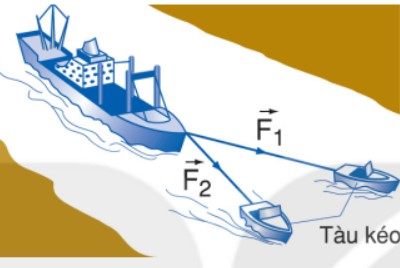
\includegraphics[width=0.35\linewidth]{../figs/VN10-2023-PH-TP014-P-1}
		\end{center}
		\begin{enumerate}[label=\alph*)]
			\item Biểu diễn các lực kéo của mỗi tàu và hợp lực tác dụng vào tàu chở hàng.
			\item Tính độ lớn của hợp lực của hai lực kéo.
			\item Nếu góc giữa hai dây cáp bằng $90^\circ$ thì hợp lực của hai lực kéo có phương, chiều và độ lớn như thế nào?
		\end{enumerate}
		
	}
	
	\hideall{
		\begin{enumerate}[label=\alph*)]
			\item Biểu diễn các lực kéo của mỗi tàu và hợp lực tác dụng vào tàu chở hàng
			
			\begin{center}
				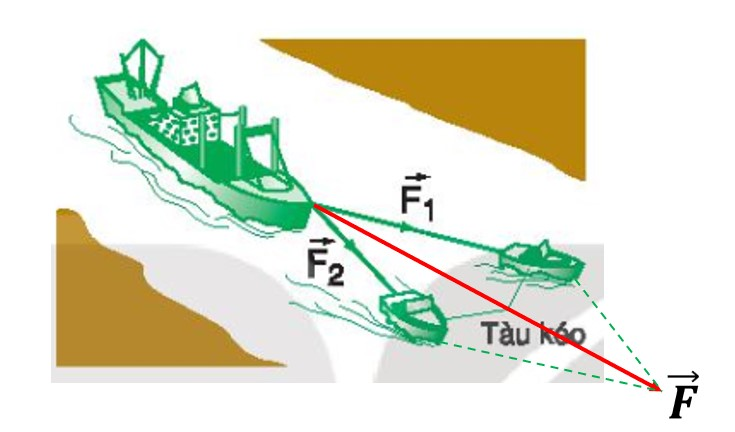
\includegraphics[scale=0.7]{../figs/VN10-2022-PH-TP015-4.jpg}
			\end{center}
			
			
			\item Độ lớn của hợp lực của hai lực kéo
			
			$$F = \sqrt{F_1^2 + F_2^2 + 2F_1F_2 \cos 30^\circ} = \SI{15454.81}{\newton}.$$
			
			\item Nếu góc giữa hai dây cáp bằng $90^\circ$ thì
			
			$$F = \sqrt{F_1^2+F_2^2} = \xsi{8000\sqrt{2}}{\newton}\approx\SI{11313.7}{\newton}.$$
			
			Hợp lực tạo với phương ngang 1 góc $45^\circ$.
		\end{enumerate}
		
	}
	
	\item \mkstar{3}
	
	{
		Một ô tô chịu một lực $F_1 = \SI{400}{N}$ hướng về phía trước và một lực $F_2 = \SI{300}{N}$ hướng về phía sau. Hỏi hợp lực tác dụng lên ô tô có độ lớn bằng bao nhiêu và hướng về phía nào?
		
		\begin{center}
			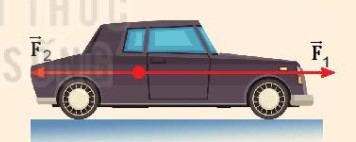
\includegraphics[scale=0.7]{../figs/VN10-2022-PH-TP015-1.jpg}
		\end{center}
		
	}
	
	\hideall{
		
		Hợp lực tác dụng lên ô tô có độ lớn là
		
		$$F = F_1 - F_2 = 400-300 = \SI{100}{N}.$$
		
		Lực $F$ cùng hướng với lực $F_1$.
		
	}

	\item \mkstar{3}
	
	{ Chất điểm chịu tác dụng đồng thời của hai lực $\vec{F}_1$ và $\vec{F}_2$ có cùng độ lớn là $10\ \text{N}$. Góc giữa hai véctơ $\vec{F}_1$ và $\vec{F}_2$  bằng $30^\circ$. Tính độ lớn của hợp lực.
	}
	\hideall{
		
		Hai lực $\vec{F_1}$  và $\vec{F_2}$ có cùng độ lớn  hợp với nhau một góc $\alpha$. 
		
		Hợp lực của chúng có độ lớn là  $$F=2F_1\cos \left( \dfrac{\alpha}{2}\right)=\text{19,3}\ \text{N} $$
	}

\item\mkstar{3}\\
Một vật chịu tác dụng đồng thời của bốn lực như hình \ref{fig:TP014-P-2}. Độ lớn của các lực lần lượt là $F_1=\SI{10}{\newton}$, $F_2=\SI{20}{\newton}$, $F_3=\SI{22}{\newton}$, $F_4=\SI{36}{\newton}$. Xác định phương, chiều và độ lớn của hợp lực do các lực này tác dụng lên vật.
\begin{center}
	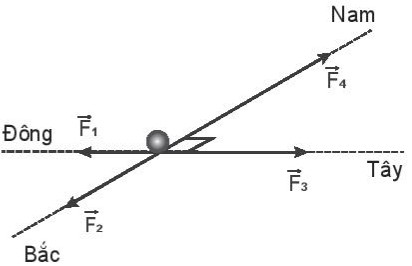
\includegraphics[width=0.35\linewidth]{../figs/VN10-2023-PH-TP014-P-2}
	\captionof{figure}{}
	\label{fig:TP014-P-2}
\end{center}
\hideall{
Hợp lực:
$$\vec{F}=\vec{F}_1+\vec{F}_2+\vec{F}_3+\vec{F}_4=\vec{F}_{13}+\vec{F}_{24}.$$
\begin{center}
	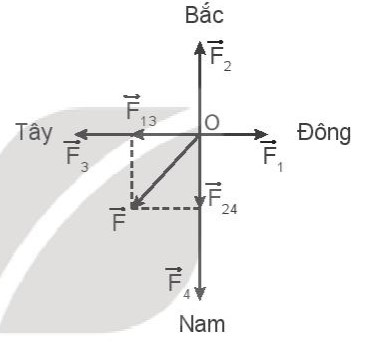
\includegraphics[width=0.35\linewidth]{../figs/VN10-2023-PH-TP014-P-3}
\end{center}
Vì $\vec{F}_1\uparrow\downarrow \vec{F}_3 \Rightarrow F_{13}=\left|F_1-F_3\right|=\SI{12}{\newton}$\\
và $\vec{F}_2\uparrow\downarrow\vec{F}_4\Rightarrow F_{24}=\left|F_2-F_4\right|=\SI{16}{\newton}$.\\
Vì $\vec{F}_{13}\bot\vec{F}_{24}$ nên độ lớn hợp lực:
$$F=\sqrt{F^2_{13}+F^2_{24}}=\sqrt{12^2+16^2}=\SI{20}{\newton}.$$
}

\item \mkstar{3}\\
Cho ba lực đồng quy, đồng phẳng $\vec{F}_1$, $\vec{F}_2$, $\vec{F}_3$ lần lượt hợp với trục $Ox$ những góc $\SI{0}{\degree}$, $\SI{60}{\degree}$, $\SI{120}{\degree}$ và độ lớn của các lực là $F_1=F_3=2F_2=\SI{30}{\newton}$. Tìm hợp lực của ba lực trên.
\hideall{
\begin{center}
	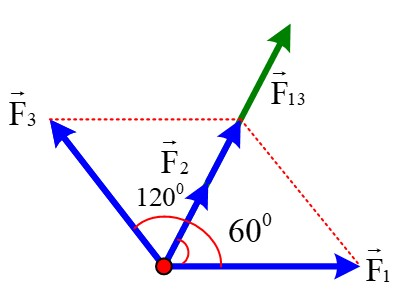
\includegraphics[width=0.3\linewidth]{../figs/VN10-2023-PH-TP014-P-4}
\end{center}
Theo đề bài ta có $\left(\vec{F}_1;\vec{F}_3\right)=\SI{120}{\degree}$ và $F_1=F_3=\SI{30}{\newton}$ nên 
\begin{equation*}
	\begin{cases}
		F_{13}=F_1=F_3=\SI{30}{\newton}\\
		\left(\vec{F}_{13};\vec{F}_1\right)=\SI{60}{\degree}
	\end{cases}
\end{equation*}
Mà $\left(\vec{F}_1;\vec{F}_2\right)=\SI{60}{\degree}$ nên $\vec{F}_{13}\uparrow\uparrow\vec{F}_2$\\
\begin{equation*}
	\Rightarrow\begin{cases}
		\vec{F}\uparrow\uparrow\vec{F}_2\\
		F=F_{13}+F_2=\SI{45}{\newton}
	\end{cases}
\end{equation*}
}

\item \mkstar{3}\\
Cho ba lực đồng quy cùng nằm trong một mặt phẳng, có độ lớn bằng nhau bằng $\SI{80}{\newton}$ và từng đôi một hợp nhau góc $\SI{120}{\degree}$. Tìm hợp lực của ba lực.
\hideall{
\begin{center}
	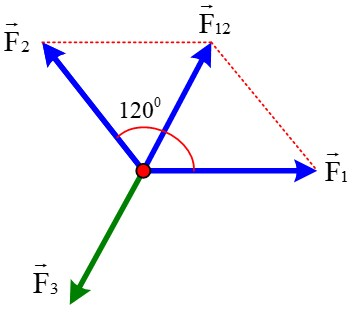
\includegraphics[width=0.35\linewidth]{../figs/VN10-2023-PH-TP014-P-5}
\end{center}
Vì $F_1=F_2$ và $\left(\vec{F}_1;\vec{F}_2\right)=\SI{120}{\degree}$ nên
\begin{equation*}
	F_{12}=F_1=F_2=\SI{80}{\newton}\\
	\left(\vec{F}_{12};\vec{F}_1\right)=\SI{60}{\degree}
\end{equation*}
Hợp lực:
$$\vec{F}=\vec{F}_1+\vec{F}_2+\vec{F}_3=\vec{F}_{12}+\vec{F}_3$$
Vì $\vec{F}_{12}\uparrow\downarrow\vec{F}_3$ nên
$$F=F_{12}-F_3=\SI{0}{\newton}.$$
}
\end{enumerate}